\documentclass[boxes]{gsypset}

% Info for header
\mailbox{}
\initials{}
\collaborators{}
\class{Math 60}
\assignment{HW 8}
\duedate{May 26, 2016}

\usepackage{caption}

\begin{document}
	\begin{problem}[5.2.7]
		Evaluate the given iterated integral.
		In addition, sketch the region $D$ that is determined by the limits of integration.
		\[
			\int_{-1}^3 \int_x^{2x+1} xy \dx{y} \dx{x}
		\]
	\end{problem}
	\begin{solution}
		
	\end{solution}
	
	\begin{problem}[5.2.14]
		Figure 5.43 shows the level curves indicating the varying depth (in feet) of a 
		\SI{25}{ft} by \SI{50}{ft} swimming pool. 
		Use a Riemann sum to estimate, to the nearest \SI{100}{ft^3}, 
		the volume of water that the pool contains.
		\begin{center}
			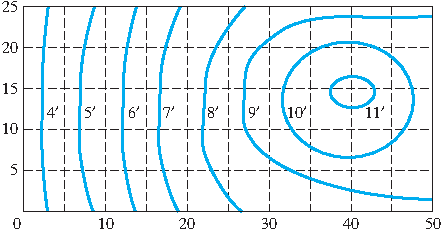
\includegraphics{img/5_2_14}
			\renewcommand{\thefigure}{5.43}
			\captionof{figure}{}
		\end{center}
	\end{problem}
	\begin{solution}
		
	\end{solution}
	
	\begin{problem}[5.3.1]
		Consider the integral
		\[
			\int_0^2 \int_{x^2}^{2x} (2x + 1) \dx{y} \dx{x}
		\]
		\begin{subproblems}
			\subproblem Evaluate this integral.
				\begin{solution}
					
				\end{solution}
			\subproblem Sketch the region of integration.
				\begin{solution}
					
				\end{solution}
			\subproblem
				Write an equivalent iterated integral with the order of integration reversed. 
				Evaluate this new integral and check that your answer agrees with part (a).
				\begin{solution}
					
				\end{solution}
		\end{subproblems}
	\end{problem}
	
	\begin{problem}[5.3.13]
		Rewrite the sum of iterated integrals as a single iterated integral by 
		reversing the order of integration, and evaluate.
		\[
			\int_0^8 \int_0^{\sqrt{\frac{y}{3}}} y \dx{x} \dx{y} +
			\int_8^{12} \int_{\sqrt{y-8}}^{\sqrt{\frac{y}{3}}} y \dx{x} \dx{y}
		\]
	\end{problem}
	\begin{solution}
		
	\end{solution}
	
	\begin{problem}[5.3.18]
		Evaluate the iterated integral
		\[
			\int_0^2 \int_{\frac{y}{2}}^1 e^{-x^2} \dx{x} \dx{y}
		\]
	\end{problem}
	\begin{solution}
		
	\end{solution}
	
	\begin{problem}[5.4.4]
		Find the value of $\iiint_W z \dx{V}$, where $W = [-1,2]\times[2,5]\times[-3,3]$,
		without resorting to explicit calculation.
	\end{problem}
	\begin{solution}
		
	\end{solution}
	
	\begin{problem}[5.4.5]
		Evaluate the iterated integral
		\[
			\int_{-1}^2 \int_1^{z^2} \int_0^{y+z} 3yz^2 \dx{x} \dx{y} \dx{z}
		\]
	\end{problem}
	\begin{solution}
		
	\end{solution}
	
	\begin{problem}[5.4.18]
		Integrate the function $f(x,y,z) = z$ over the region $W$ bounded by
		$z = 0$, $x^2 + 4y^2 = 4$, and $z = x + 2$.
	\end{problem}
	\begin{solution}
		
	\end{solution}
	
	\begin{problem}[5.4.29ab]
		Consider the iterated integral
		\[
			\int _{-2} ^2
				\int _0 ^{\frac{1}{2} \sqrt{4 - x^2}}
					\int _{x^2 + 3y^2} ^{4 - y^2}
						(x^3+y^3)
					\dx{z}
				\dx{y}
			\dx{x}
		\]
		\begin{subproblems}
			\subproblem
				This integral is equal to a triple integral over a solid region $W$ in $\mathbb{R}^3$.
				Describe $W$.
				\begin{solution}
					
				\end{solution}
			\subproblem
				Set up an equivalent iterated integral by integrating first with respect to z, 
				then with respect to x, then with respect to y. 
				Do not evaluate your answer.
				\begin{solution}
					
				\end{solution}
		\end{subproblems}
	\end{problem}
\end{document}